%\frame{\titlepage}

\section{Kommunikation}
\begin{frame}
\tableofcontents[currentsection]
\end{frame}
%\frame{\tableofcontents}
%\section{Einleitung}

\subsection{Einleitung}
\frame
{
  \frametitle{Einleitung}
  \begin{itemize}
    \item Zur Koordination haben die NAOs die M\"oglichkeit, miteinander zu kommunizieren.
  \end{itemize}
  %\begin{center}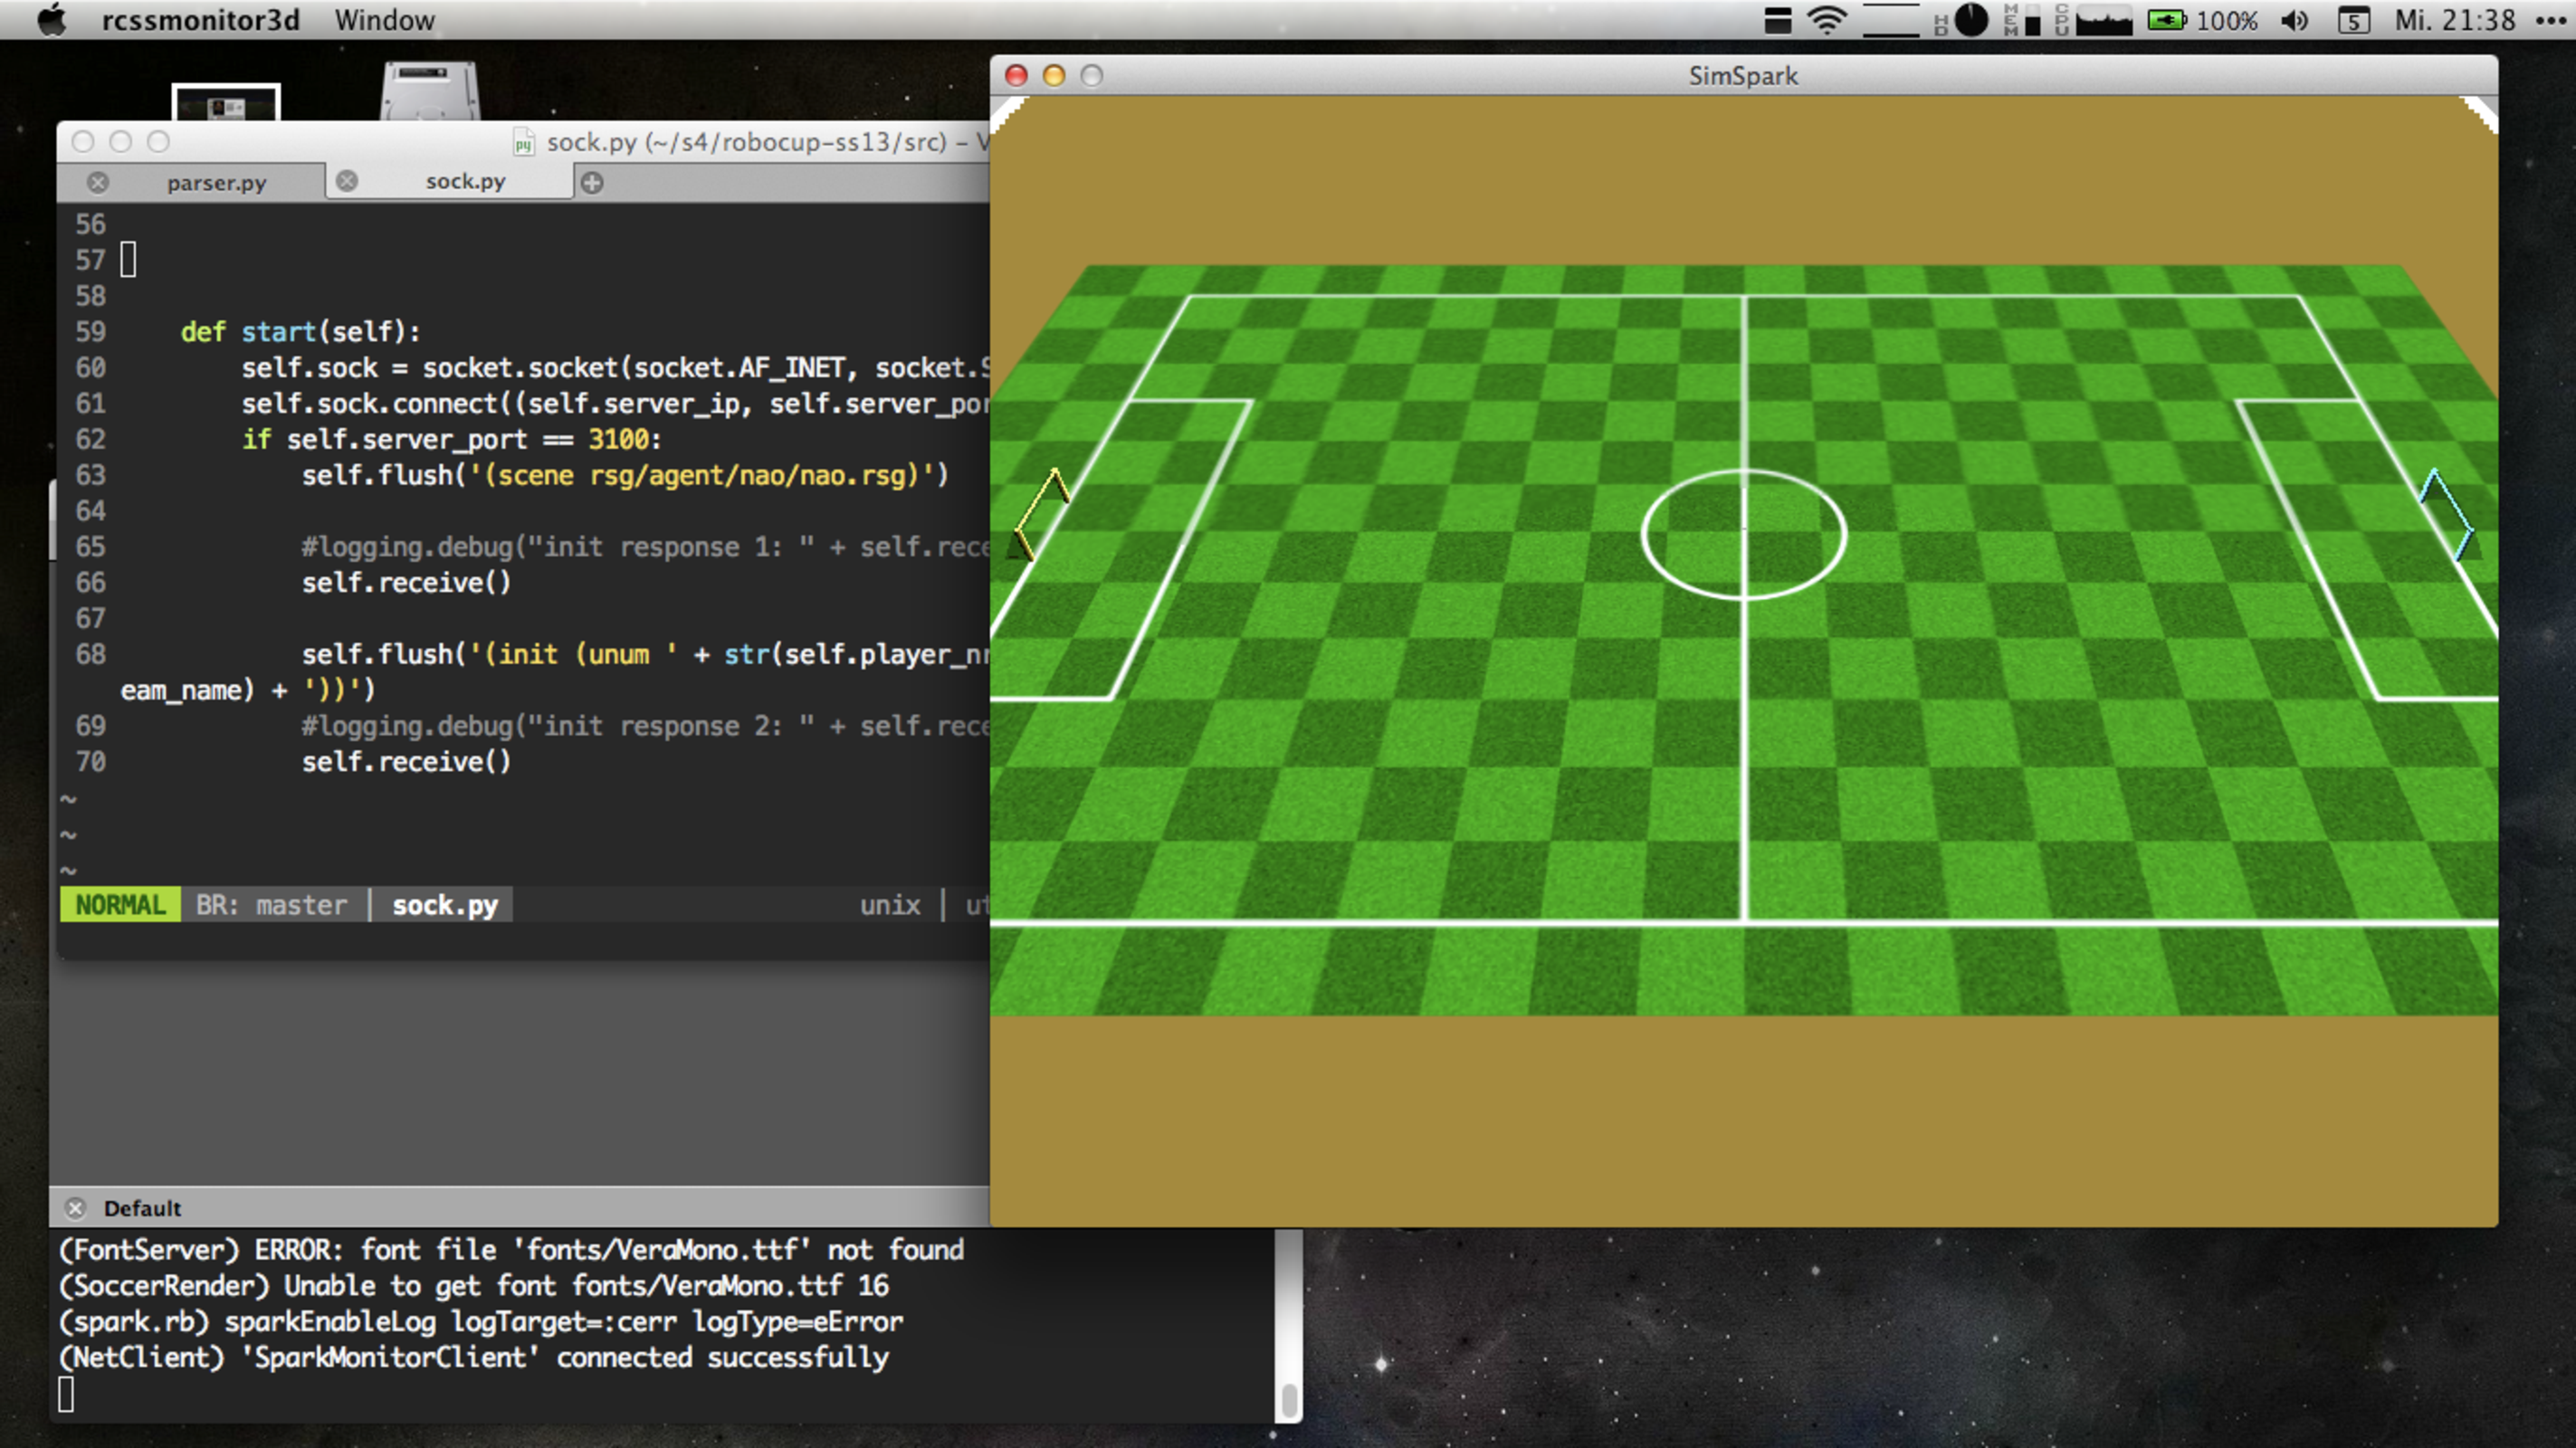
\includegraphics[height=5cm, center]{simulator.pdf}\end{center}
}
  
\frame
{
  \frametitle{Einleitung}
  \begin{itemize}
    \item<1-> Das funktioniert, im Prinzip, wie bei Menschen auch:
    \item<2-> Zun\"achst wird die Nachricht erstellt und codiert.
    \item<3-> \"Uber den Server wird sie nun an die NAOs weitergeleitet.
    \item<4-> Diese m\"ussen die Nachricht entschl\"usseln und interpretieren.
  \end{itemize}
  
  \begin{center}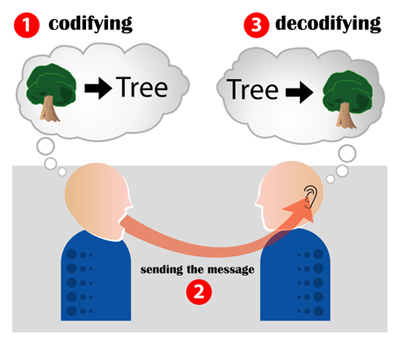
\includegraphics[height=5cm, center]{Encoding_communication.jpg}\end{center}
}

\frame
{
  \frametitle{Die Rahmenbedingungen}
  \begin{itemize}
    \item<1-> Die Kommunikation unterliegt einigen Einschr\"ankungen: \vskip0.5cm
    \item<2-> Maximal 20 Zeichen pro Nachricht.
    \item<3-> Es steht nur ein eingeschr\"ankter ASCII-Zeichensatz zur Verf\"ugung. (90 Zeichen)
  \end{itemize}
}

\subsection{Codierung}
%\section{Parser}
\frame
{
  \frametitle{Codierung}
  
  \begin{itemize}
    \item<1-> \"Uber say-Methoden kann eine Nachricht codiert werden.
    \item<2-> Eine codierte Nachricht ist wie folgt aufgebaut: \vskip0.5cm
    \item<3-> $<MessageCode><Parameter><Pr\ddot{u}fsumme>$ \vskip0.5cm
    \item<4-> Ein Message-Code definiert hier die Art der Nachricht.
    \item<5-> Sender, Empf\"anger und Parameter sind dahinter angeh\"angt. \\Doubles als Parameter haben einen Wertebereich von $\pm$364.00.
    \item<6-> Am Ende wird die Nachricht durch eine Pr\"ufsumme validiert.
  \end{itemize}
}

\subsection{Senden und Empfangen}
%\section{Probleme}
\frame
{
  \frametitle{Senden der Nachricht}
  
  \begin{itemize}
    \item<1-> Nachdem die Nachricht codiert ist, kann sie versendet werden.
    \item<2-> Hierzu steht einem der Say-Effector des NAO zur Verf\"ugung.
    \item<3-> \"Uber ihn gelangt die Nachricht an den Server.
  \end{itemize}
}

\frame
{
  \frametitle{Empfangen der Nachricht}
  
  \begin{itemize}
    \item<1-> Nun muss die Nachricht nat\"urlich auch empfangen werden.
    \item<2-> Daf\"ur nutzen wir den Hear-Perceptor des NAO.
    \item<3-> Wenn der NAO gerade zuh\"ort, empf\"angt er \"uber ihn die Nachricht.
    \item<4-> Hierf\"ur steht eine Methode hear(...) zur Verf\"ugung.
  \end{itemize}
}

\subsection{Decodierung}
\frame
{
  \frametitle{Decodierung}
  
  \begin{itemize}
    \item<1-> Zun\"achst wird die Nachricht von einem Translator in ihre Bestandteile aufgetrennt.
    \item<2-> Daraus wird ein HearObject erstellt.
    \item<3-> Dieses unterscheidet sich je nach Nachricht, und alle relevanten Daten sind in ihm gespeichert.
    \item<4-> \"Uber eine eval()-Methode kann das Objekt nun ausgewertet werden. (Taktik)
  \end{itemize}
}

\subsection{Fazit}
\frame
{
  \frametitle{Weitere Details}
  
  \begin{itemize}
    \item<1-> Es gibt noch einige weitere Einschr\"ankungen der Kommunikation, die zu beachten sind: \vskip0.5cm
    \item<2-> Ein NAO ist 50m weit zu h\"oren.
    \item<3-> Er kann ausserdem nur alle 0.04s etwas h\"oren. In der Zwischenzeit kann er keine Nachrichten empfangen.
    \item<4-> Sollten 2 NAOs gleichzeitig sprechen, wird nur einer von ihnen geh\"ort. Der Sprecher h\"ort sich jedoch immer selbst.
    \item<5-> Die Teams sprechen versetzt, man kann also nicht die Kommunikation des anderen Teams blockieren.
  \end{itemize}
}

\frame
{
  \frametitle{Zusammenfassung}

  \begin{itemize}
    \item<1-> Communication.py stellt Methoden zur Kommunikation zur Verf\"ugung.
    \item<2-> say-Methoden dienen dem senden von Nachrichten.
    \item<3-> Soll der NAO zuh\"oren was gesagt wird, benutzt man hear().
    \item<4-> Man erh\"alt nun ein HearObject.
    \item<5-> \"Uber eval() wertet man es zu einem geeigneten Zeitpunkt aus.
  \end{itemize}
}